\section{Applications}

We investigated the applications of our model across various domains. The model's ability to generate coherent and contextually relevant text makes it suitable for question-answering tasks with a chatbot.



\subsection{Chatbot Application}

We used Gemini 2.5 Flash~\cite{comanici2025gemini} to create a chatbot that can answer questions based on the provided context. The chatbot is designed to understand and respond to user queries in a conversational manner, leveraging the model's capabilities to generate human-like responses.

The system operates in a two-stage process: context generation followed by user interaction. The first stage is initiated upon video upload. The system automatically subjects the video to a multi-modal analysis pipeline involving four concurrent modules: a video captioning model for action summaries, a keyframe captioning model for scene details, an object detection model for itemized lists, and a speech recognition model for audio transcription. The information from these sources is aggregated into a unified contextual document. In the second stage, the user can query the chatbot, which operates exclusively on this pre-generated context to deliver precise answers without re-processing the video.

\subsection{Video Captioning Implementation}

To generate a dynamic, event-based understanding of the video, we first partition the input video into continuous 20-second segments. Each segment is then fed into the video captioning model, which produces a concise description of the main actions and events occurring within that timeframe. The resulting sequence of captions provides a narrative summary that serves as the primary context for the chatbot.


\subsection{Keyframe Captioning Implementation}

To complement the action-based summaries, we implement keyframe captioning to capture static, high-fidelity visual details. The pipeline begins by extracting keyframes from the video, which are frames chosen to represent distinct visual states or significant changes in the scene. Each of these keyframes is then individually analyzed by our image captioning model, generating a rich, scene-specific description. This provides a granular level of detail that the broader video summary might omit.


\subsection{Enhancing Context with Object Detection}

While our captioning models provide high-level summaries of scenes and actions, they may not always capture specific details about every object present in the video. A caption might say, ``\textit{A person is working in an office}'', but it might not list the specific items on the desk, such as a laptop, a mug, or a phone.

To create a more detailed and robust context for our chatbot, we integrated an \textbf{object detection} model. For this task, we chose the \textbf{Ultralytics YOLOv11}~\cite{yolo11_ultralytics} model, using a version pre-trained on the comprehensive \textbf{COCO dataset}. This model is highly efficient and accurate at identifying a wide range of common objects.

The integration process is designed to complement our existing workflow. The same keyframes that are sent to the image captioning model are also processed by YOLOv11. The output from YOLO is a list of all detected objects within those frames. This list is then added to the overall context that is fed to the chatbot.


\subsection{Enhancing Context with Speech Recognition}

To capture the auditory information within the video, we integrated an automatic speech recognition (ASR) module. For this purpose, we selected PhoWhisper~\cite{le2024phowhisper}, a state-of-the-art model specifically fine-tuned for the Vietnamese language. Based on OpenAI's robust Whisper architecture, PhoWhisper is trained on a large and diverse dataset of Vietnamese accents, ensuring high accuracy for transcription.

The integration process is straightforward: the audio stream is first extracted from the input video and then processed by the PhoWhisper model. The output is a complete text transcript of any spoken dialogue. This transcript is then added to the overall context fed to the chatbot, allowing it to understand and answer questions based on what is said in the video.


\subsection{Serving Architecture \& Request Flow}

\begin{figure}[H]
    \centering
    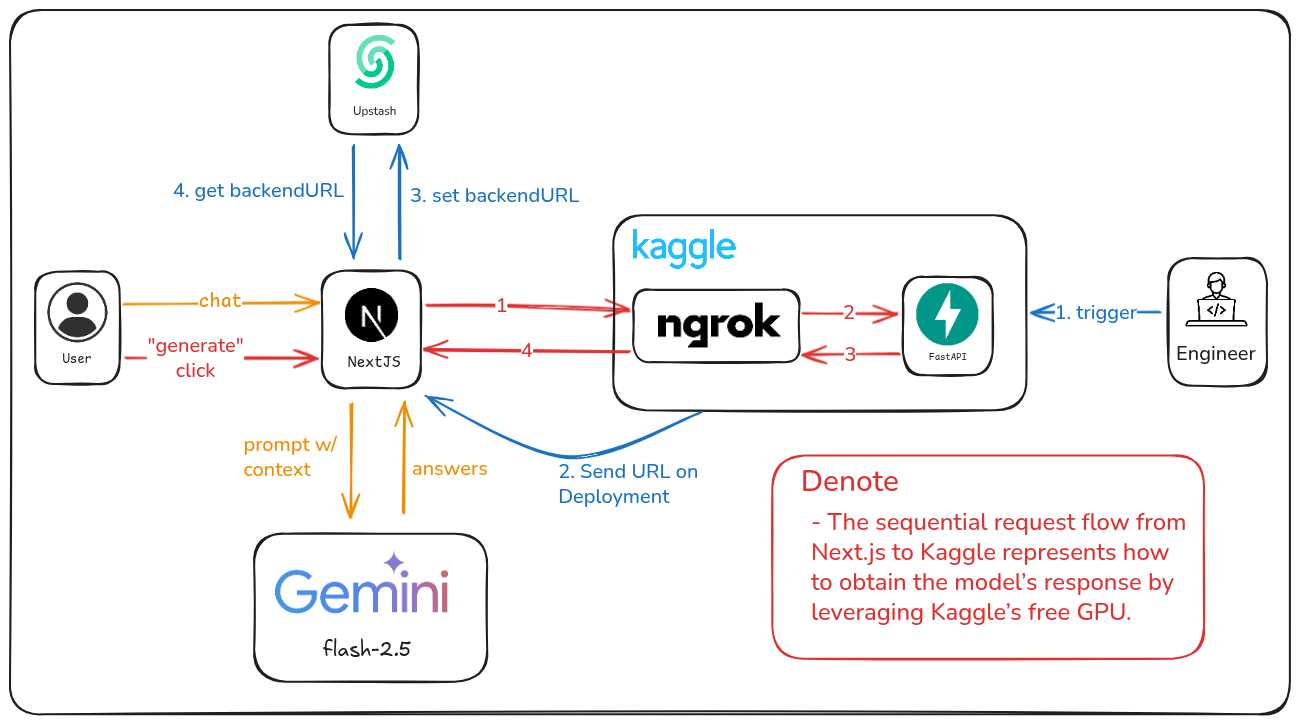
\includegraphics[width=0.9\textwidth]{image/high-level-architecture.png}
    \caption{Deployment \& Request Flow (Next.js $\Leftrightarrow$ Kaggle GPU)}
    \label{fig:deployment-flow}
\end{figure}

Figure~\ref{fig:deployment-flow} summarizes how the web app serves requests using a lightweight Next.js frontend and a GPU-backed FastAPI service running on Kaggle via ngrok, alongside Gemini~2.5 Flash for conversational reasoning.

\textbf{Provisioning (blue):}
\begin{enumerate}
    \item An engineer launches the FastAPI service on Kaggle, which is exposed to the Internet through ngrok and yields a public URL.
    \item That URL is sent back to the app on deployment.
    \item The app stores the URL as \texttt{backendURL} in Upstash.
    \item At runtime, the Next.js client reads \texttt{backendURL} from Upstash so it always targets the current backend.
\end{enumerate}

\textbf{Inference at runtime (red/orange):}
\begin{enumerate}
    \item When the user clicks \textbf{Generate}, Next.js calls the Kaggle \texttt{backendURL} through ngrok.
    \item Ngrok forwards the request to FastAPI on the GPU.
    \item FastAPI returns the result to ngrok.
    \item The response is delivered back to Next.js.
\end{enumerate}

In parallel, Next.js sends the prompt plus context to \textbf{Gemini 2.5 Flash} and combines the LLM's answer with the GPU model's outputs to reply to the user. 

This setup keeps the UI simple, hides the transient Kaggle URL behind Upstash, and lets the system leverage Kaggle's free GPU without operating dedicated servers.



\subsection{User Interface}

% We designed a user-friendly interface for the chatbot, allowing users to interact with it easily. The interface includes a video player for watching the video, a text input box for entering questions, and a chat window for displaying the chatbot's responses. This setup ensures a seamless user experience, enabling users to engage with the chatbot while watching the video.


\begin{figure}[H]
\centering
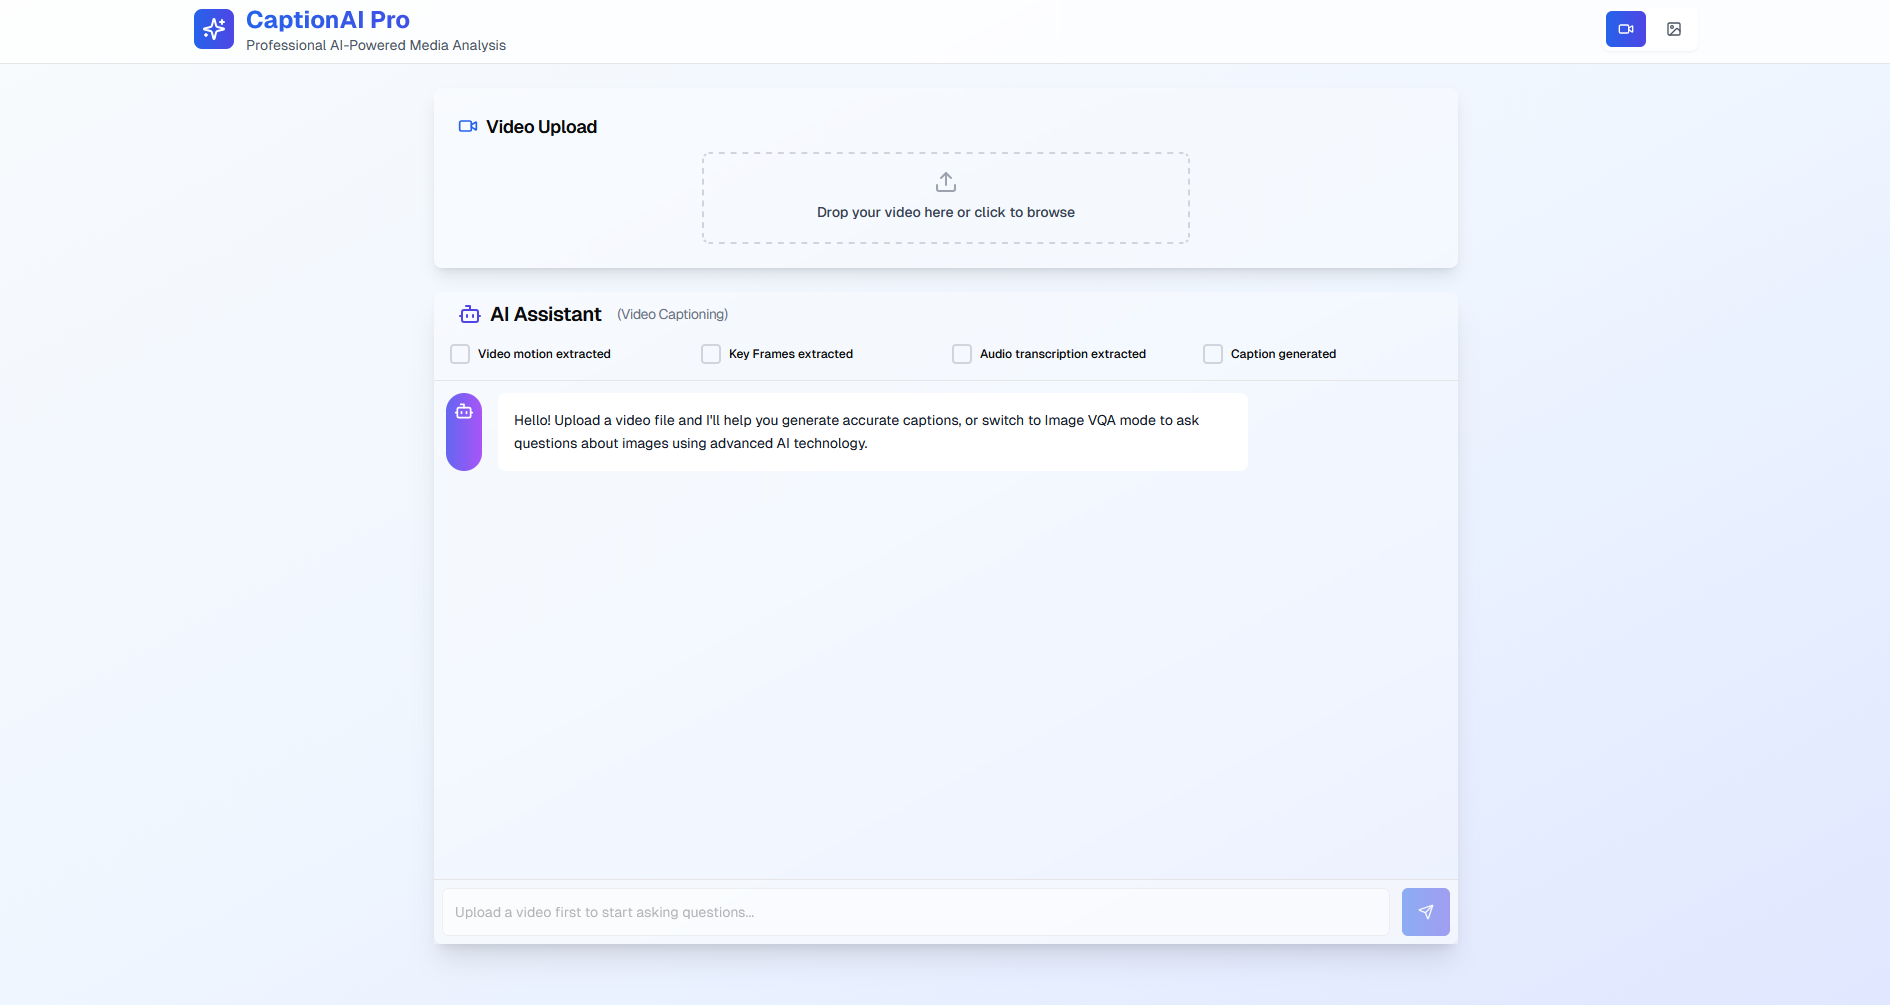
\includegraphics[width=0.9\textwidth]{image/UI/home.png}
\caption{User interface of the our application before uploading video.}
\label{fig:home_ui}
\end{figure}

\begin{figure}[H]
\centering
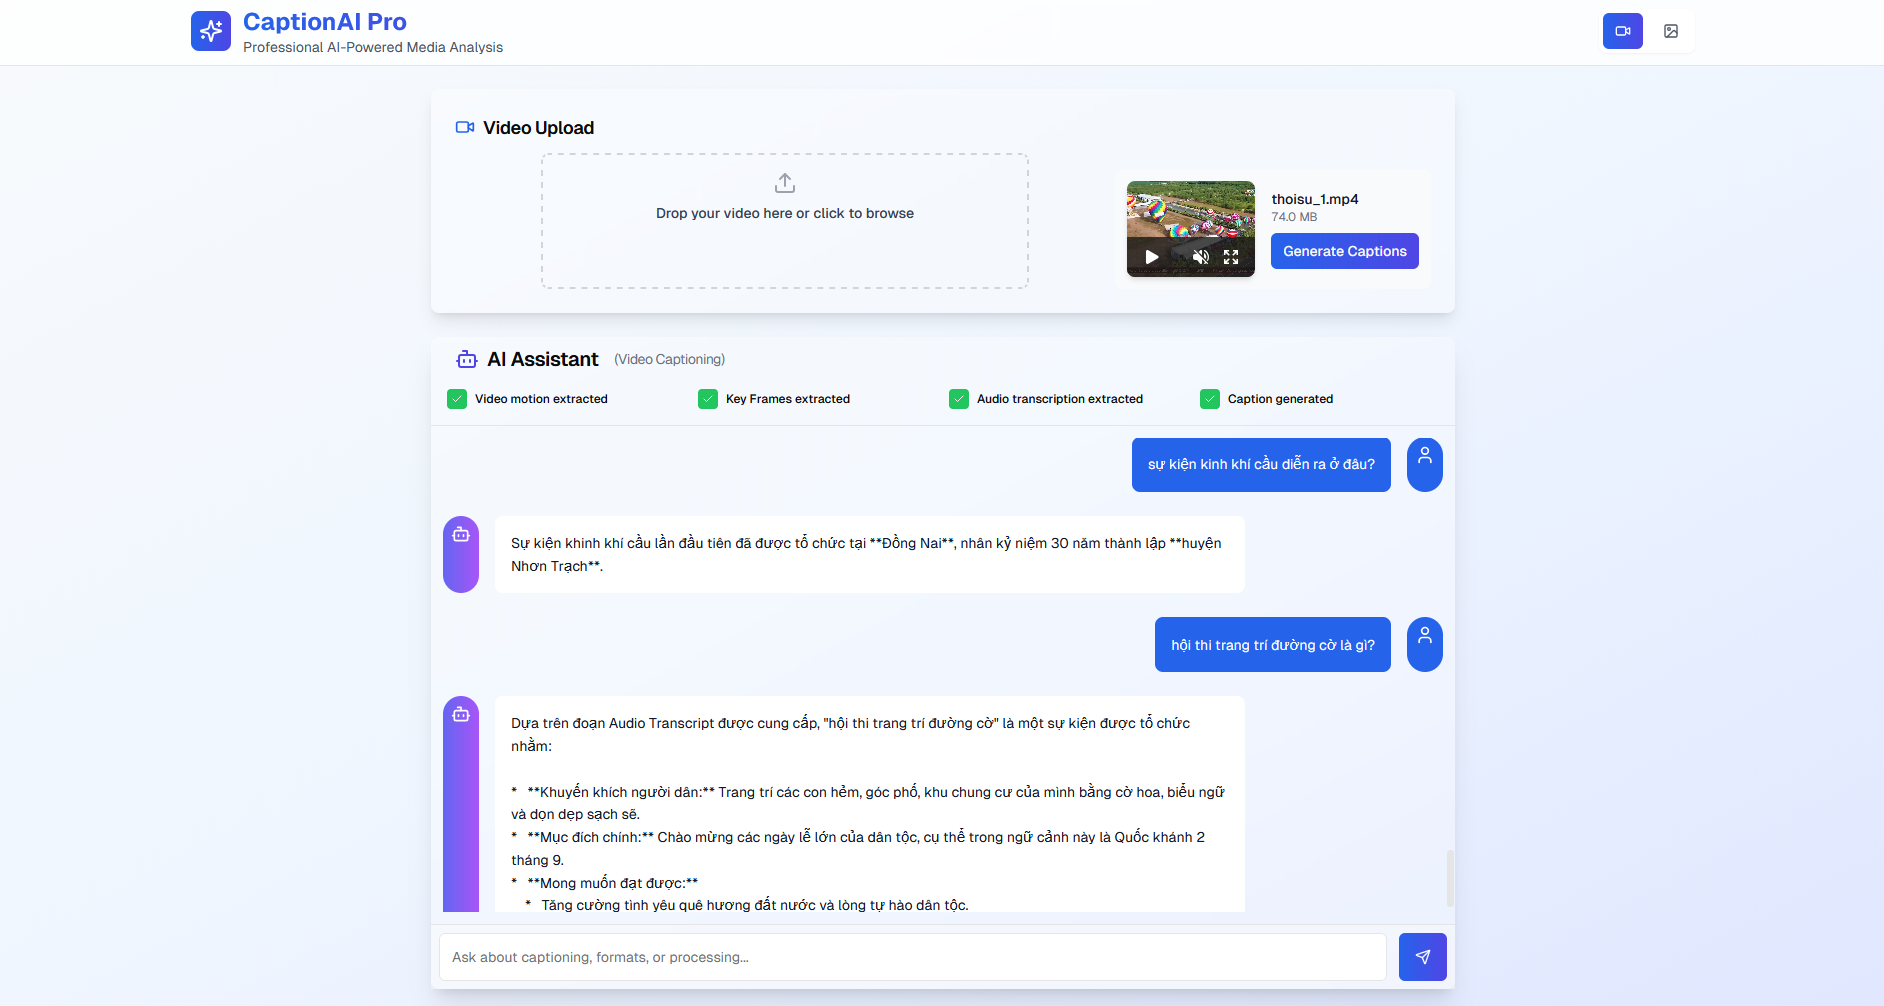
\includegraphics[width=0.9\textwidth]{image/UI/example.png}
\caption{Example of user--chatbot interaction.}
\label{fig:example_ui}
\end{figure}

